\documentclass[a4paper,12pt]{report}

%Русский язык
\usepackage[T2A]{fontenc}
\usepackage[utf8]{inputenc}
\usepackage[english,russian]{babel}
\usepackage{cmap}

%Работа с кодом
\usepackage{listings}
\usepackage{color}

\definecolor{green}{rgb}{0,0.6,0}
\definecolor{gray}{rgb}{0.5,0.5,0.5}
\definecolor{red}{rgb}{0.6,0,0}

\lstset{
        language=Python, 
        basicstyle=\small\ttfamily, 
        numberstyle=\tiny,           
        columns=flexible,
        stepnumber=1,                   
        numbersep=5pt,        
        showspaces=false,
        showstringspaces=false,
        showtabs=false,
        tabsize=2,                
        captionpos=b,              
        breaklines=true,           
        breakatwhitespace=false,
        keywordstyle=\color{green},
        commentstyle=\color{gray},
        stringstyle=\color{red},      
}

%Математика
\usepackage{amsmath,amsfonts,amssymb,amsthm,mathtools} 

%Изображения
\usepackage{float}
\usepackage{graphicx}
\graphicspath{ {./img/} }

%Поля страницы
\usepackage{geometry} 
\geometry{left=2.3cm} 
\geometry{right=1.8cm} 
\geometry{top=2cm} 
\geometry{bottom=2.5cm} 

%Отступы
\usepackage{indentfirst}
\setlength{\parskip}{0cm}

\begin{document} 

\begin{titlepage}
\newpage
	\begin{center}
		\large Санкт-Петербургский политехнический университет Петра Великого\\
		Институт компьютерных наук и технологий\\
		Высшая школа интеллектуальных систем и суперкомпьютерных технологий\\
	\end{center}
\vspace{7cm}

\begin{center}
		\large \textbf{Отчёт по лабораторной работе №10} \\
		\textbf{Дисциплина:} Телекоммуникационные технологии\\
		\textbf{Тема:} Линейные стационарные системы
\end{center}
\vspace{4cm}
	
\begin{flushright}
		\large Работу выполнил:\\ Ляшенко В.В.\\
		Группа: 3530901/80201\\
		Преподаватель:\\ Богач Н.В.
\end{flushright}

\vspace{\fill}
\begin{center}
	\large Санкт-Петербург\\ 2021
	\end{center}
\end{titlepage}

\tableofcontents
\listoffigures
\lstlistoflistings

\chapter{Упражнение 10.1}
    В разделе "Акустическая характеристика" используется круговая свёртка, в результате которой можно заметит, что на выходе, в начале фрагмента, слышна лишняя нота, "затекшая" из конца этого фрагмента. 
    
    Решить эту проблему можно, если перед вычислением ДПФ добавить достаточно нулей в конец сигнала. Тогда эффекта "заворота" получится избежать.
    
    Изменим пример \texttt{chap10.ipynb} и убедимся, что дополнение нулями устраняет лишнюю ноту в начале фрагмента.
    
    Сократим оба сигнала до $2^{16}$ элементов, а затем дополню их нулями до $2^{17}$.
    
\section{Выстрел}      
    Начнём с сигнала выстрела (Рис.1.1).
\begin{lstlisting}[caption=Дополнение нулями]
       from thinkdsp import read_wave

       response = read_wave('180960__kleeb__gunshot.wav')

       start = 0.12
       response = response.segment(start=start)
       response.shift(-start)

       response.truncate(2**16)
       response.zero_pad(2**17)

       response.normalize()
       response.plot()
       decorate(xlabel='Time (s)')
\end{lstlisting}
\begin{figure}[H]
        \centering
        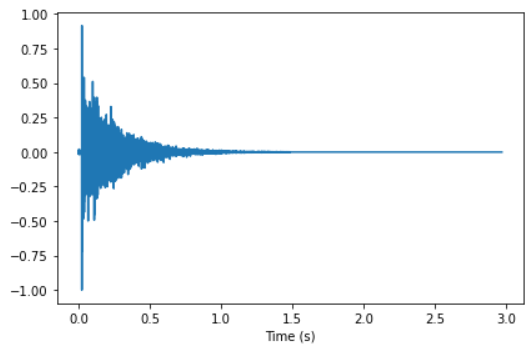
\includegraphics[width=0.8\textwidth]{fig1-1.PNG}
        \caption{Сигнал выстрела}
        \label{fig:fig1-1}
\end{figure}

    Его спектр будет следующим (Рис.1.2).
\begin{lstlisting}[caption=Получение спектра сигнала]
       transfer = response.make_spectrum()
       transfer.plot()
       decorate(xlabel='Frequency (Hz)', ylabel='Amplitude')
\end{lstlisting}
\begin{figure}[H]
        \centering
        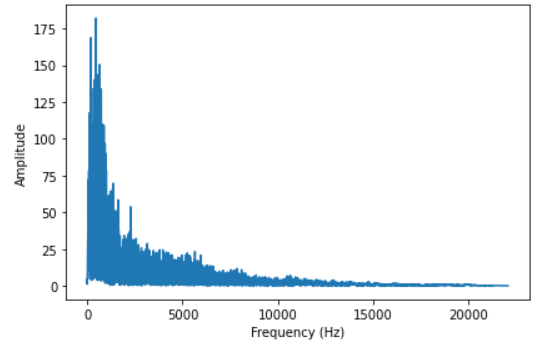
\includegraphics[width=0.8\textwidth]{fig1-2.PNG}
        \caption{Спектр сигнала выстрела}
        \label{fig:fig1-2}
\end{figure}   

\section{Скрипка}
    Теперь проделаем тоже самое для скрипки (Рис.1.3).
\begin{figure}[H]
        \centering
        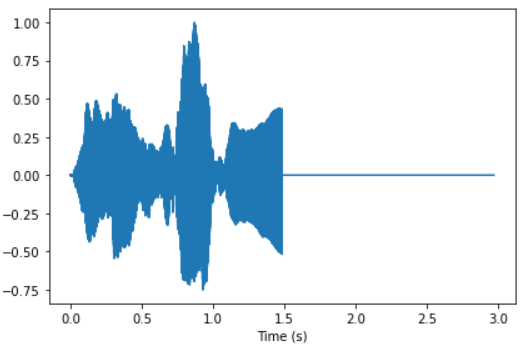
\includegraphics[width=0.8\textwidth]{fig1-3.PNG}
        \caption{Сигнал скрипки}
        \label{fig:fig1-3}
\end{figure} 

    Получим спектр сигнала (Рис.1.4).
\begin{lstlisting}[caption=Получение спектра сигнала]
       spectrum = violin.make_spectrum()
       output = (spectrum * transfer).make_wave()
       output.normalize()
       output.plot()
\end{lstlisting}
\begin{figure}[H]
        \centering
        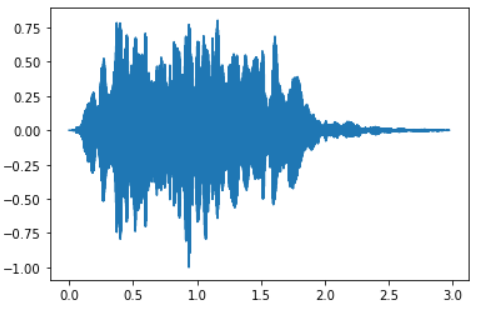
\includegraphics[width=0.8\textwidth]{fig1-4.PNG}
        \caption{Спектр сигнала скрипки}
        \label{fig:fig1-4}
\end{figure}  
       
    При прослушивании получившегося сигнала мы убеждаемся, что "затекшей" ноты в начале больше нет.

\chapter{Упражнение 10.2}
\section{Импульсная характеристика}
    Скачаем из библиотеки Open AIR импульсную характеристику. Это будет запись из женского клуба с частотой дискретизации 44100 (Рис.2.1). 
\begin{lstlisting}[caption=Получение сигнала]
       response = read_wave('sounds/spokane_womans_club_ir.wav')

       start = 0
       duration = 5
       response = response.segment(duration=duration)
       response.shift(-start)

       response.normalize()
       response.plot()
       decorate(xlabel='Time (s)')
\end{lstlisting}
\begin{figure}[H]
        \centering
        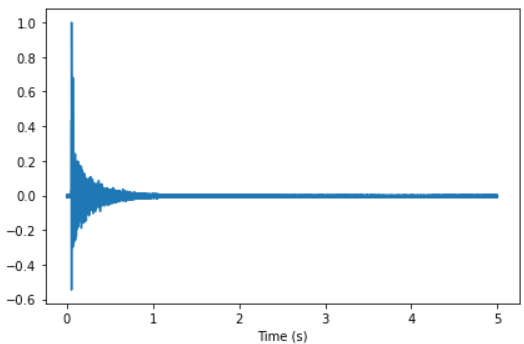
\includegraphics[width=0.8\textwidth]{fig2-1.PNG}
        \caption{Полученный сигнал}
        \label{fig:fig2-1}
\end{figure}  
    
    Получим спектр данного сигнала (Рис.2.2). 
\begin{figure}[H]
        \centering
        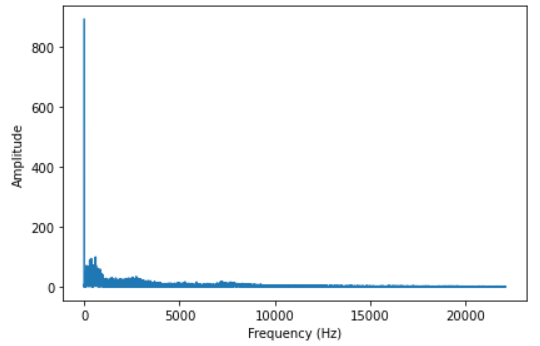
\includegraphics[width=0.8\textwidth]{fig2-2.PNG}
        \caption{Спектр полученного сигнала}
        \label{fig:fig2-2}
\end{figure}   
    
    И его логарифмическое представление (Рис.2.3).
\begin{figure}[H]
        \centering
        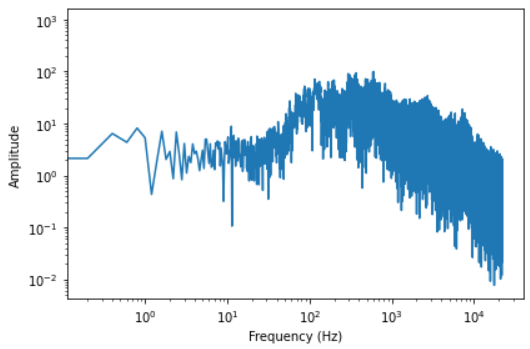
\includegraphics[width=0.8\textwidth]{fig2-3.PNG}
        \caption{Логарифмическое представление спектра}
        \label{fig:fig2-3}
\end{figure}

\section{Работа с записью}
    
    Найдём короткую запись с такой же частотой дискретизации. Получилось найти запись с игрой на пианино (Рис.2.4).
\begin{lstlisting}[caption=Получение сигнала пианино]
       wave = read_wave('sounds/186942__lemoncreme__piano-melody.wav')

       start = 0.0
       wave = wave.segment(start=start)
       wave.shift(-start)

       wave.truncate(len(response))
       wave.normalize()
       wave.plot()
       decorate(xlabel='Time (s)')
\end{lstlisting}
\begin{figure}[H]
        \centering
        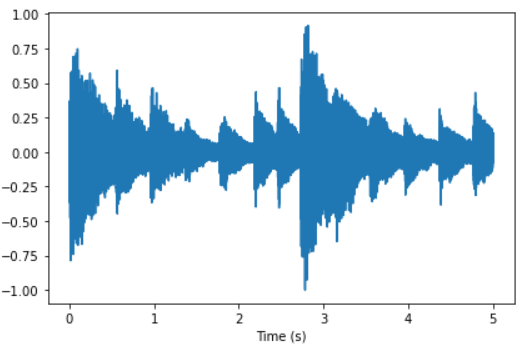
\includegraphics[width=0.8\textwidth]{fig2-4.PNG}
        \caption{Полученный сигнал пианино}
        \label{fig:fig2-4}
\end{figure}

    Обрежем запись пианино до той же длины, что и у импульсной характеристики. 
\begin{lstlisting}[caption=Сокращение длины записи пианино]
       spectrum = wave.make_spectrum()
       len(spectrum.hs), len(transfer.hs)
\end{lstlisting} 
\subsection{Умножение ДПФ на фильтр}
    Смоделируем звучание пианино в пространстве с помощью умножения ДПФ записи на вычисленный фильтр, соответствующий импульстной характеристики.
\begin{lstlisting}[caption=Умножение ДПФ на фильтр]
       output = (spectrum * transfer).make_wave()
       output.normalize()
\end{lstlisting}
    
    Построим графики до обработки (Рис.2.5) и после (Рис.2.6).
\begin{figure}[H]
        \centering
        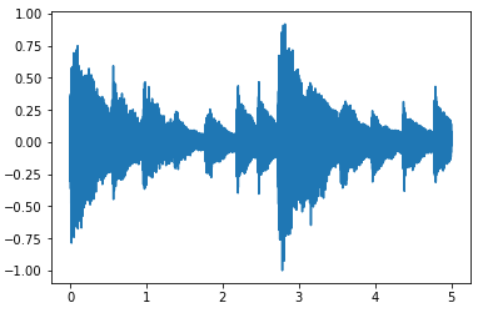
\includegraphics[width=0.8\textwidth]{fig2-5.PNG}
        \caption{Пианино до обработки}
        \label{fig:fig2-5}
\end{figure}
\begin{figure}[H]
        \centering
        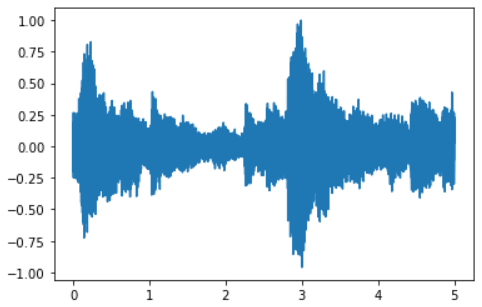
\includegraphics[width=0.8\textwidth]{fig2-6.PNG}
        \caption{Пианино после обработки}
        \label{fig:fig2-6}
\end{figure} 

    Послушаем получившуюся запись. Звук пианино действительно звучит в том женском клубе.
\subsection{Свёртка записи с импульсной характеристикой}
    
    Теперь воспользуемся свёрткой.
\begin{lstlisting}[caption=Свёртка]
       convolved = wave.convolve(response)
       convolved.normalize()
       convolved.make_audio()
\end{lstlisting}
    
    Звучит так же, как и в предыдущем случае.       
\chapter{Выводы}
    В результате выполнения данной работы мы изучили линейные стационарные системы.
   
    Также мы научились моделировать звучание в пространстве двумя способами: свёрткой записи с импульсной характеристикой и умножением ДПФ записи на вычисленный фильтр, соответствующий импульсной характеристике.
\end{document}